\documentclass[a4paper]{article}

\usepackage[spanish]{babel}
\usepackage{graphicx}
\usepackage{amsmath, amssymb}
\usepackage[margin=2cm]{geometry}
\usepackage{fancyhdr}
\usepackage{enumerate}
\usepackage[shortlabels]{enumitem}
\usepackage{parskip}
\usepackage[most]{tcolorbox}
\usepackage[hidelinks]{hyperref}
\usepackage{float}


% cabecera
\pagestyle{fancy}
\fancyhead[l]{Daniel Soto}
\fancyhead[c]{Problemas de Astronomía \#1}
\fancyhead[r]{\today}
\fancyfoot[c]{\thepage}
\renewcommand{\headrulewidth}{0.2pt} % linea horizontal

%% Definicion de comandos para formato de unidades fisicas %%
\newcommand{\m}{\text{m}}
\newcommand{\cm}{\text{cm}}
\newcommand{\km}{\text{km}}
\newcommand{\s}{\text{s}}
\newcommand{\N}{\text{N}}
\newcommand{\g}{\text{g}}
\newcommand{\kg}{\text{kg}}
\newcommand{\Msolar}{\text{M}_\odot}
\newcommand{\Mterrestre}{\text{\text{M}_\oplus}}
\newcommand{\AU}{\text{AU}}
\newcommand{\ly}{\text{ly}}
\newcommand{\nT}{\text{nT}}
\newcommand{\keV}{\text{keV}}
\newcommand{\MeV}{\text{MeV}}
\newcommand{\GeV}{\text{GeV}}
\newcommand{\atoms}{\text{atoms}}
\newcommand{\K}{\text{K}}
\newcommand{\J}{\text{J}}
\newcommand{\particles}{\text{particles}}
\newcommand{\protones}{\text{p}^+}
\newcommand{\electrones}{\text{e}^-}

\newcounter{problema}

\newtcolorbox[use counter=problema]{problema}[1][]{%
	breakable,
    colback=gray!15,
    colframe=gray!60,
    fonttitle=\bfseries,
    title={Problema~\theproblema:},
    boxrule=0.5mm,
    arc=3mm,
    boxsep=5pt,
    left=8pt,
    right=8pt,
    top=6pt,
    bottom=6pt,
    #1
}


\begin{document}

Los cinturones de Van Allen fueron descubiertos aproximadamente en 1958 cuando los satélites Explorer 1 y 3, equipados con contadores Geiger, detectaron nubes de \textit{radiactividad} dentro de los $50 000 \km$ de la Tierra. Investigaciones posteriores identificaron finalmente cuatro componentes: dos cinturones internos, compuestos por electrones de alta energía ($\sim100 \keV$) y protones (de $100 \keV$ a $400 \MeV$); un cinturón externo compuesto principalmente por electrones de alta energía (de $0.1$ a $10 \MeV$); y una región generalmente vacía llamada Zona Slot que separa estos dos sistemas de partículas.


    \begin{figure}[H]
        \centering
        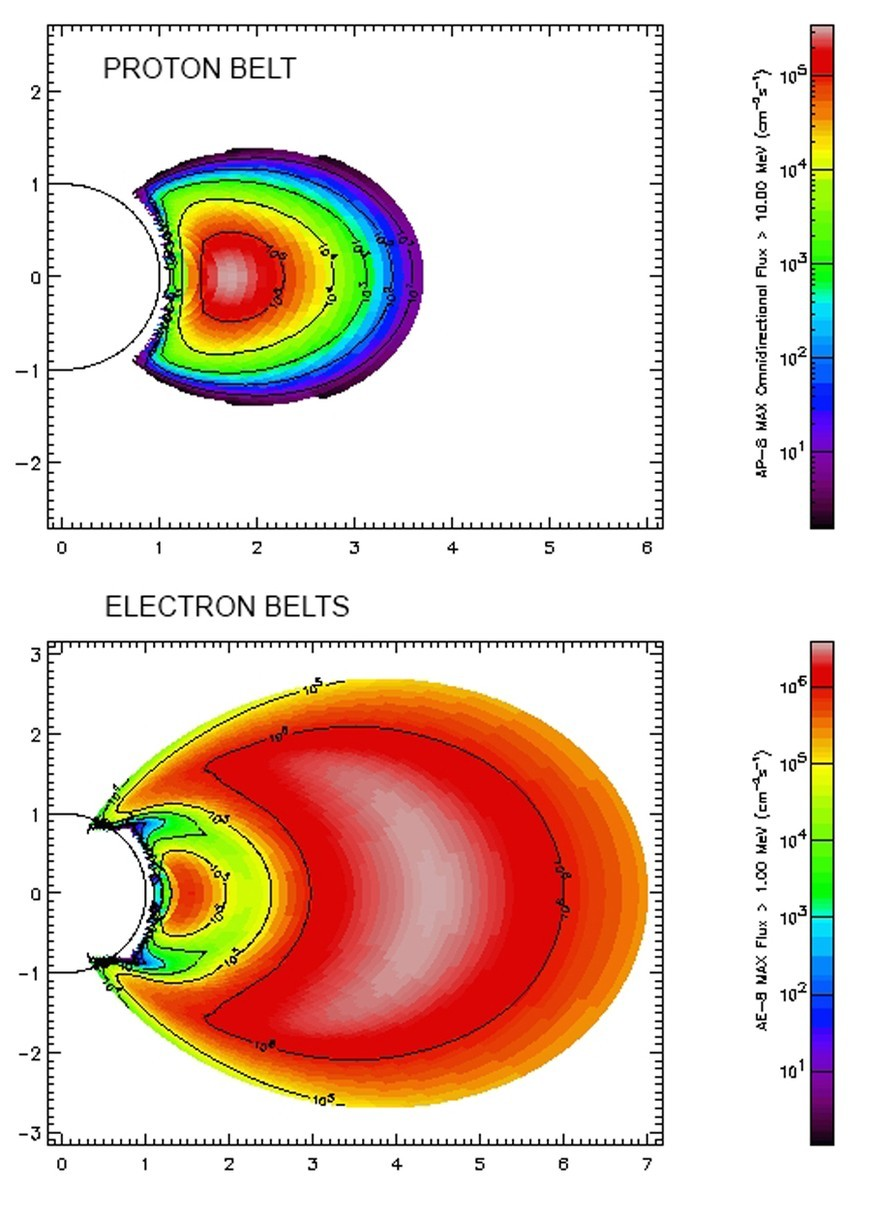
\includegraphics[width=0.7\textwidth]{test.jpg}
%        \caption{test}
        \label{fig:1}
    \end{figure}

A diferencia de otros sistemas físicos como la atmósfera terrestre al nivel del mar ($1.29 \kg/\m ^3$) o incluso el viento solar ($5 \atoms/\cm ^3$), la densidad de los cinturones de Van Allen no está muy bien definida. El número de partículas presentes en cualquier momento varía órdenes de magnitud dependiendo del tipo de partícula (electrones o protones), sus energías (de $1 \keV$ a $400 \MeV$) y el nivel de actividad solar.

Dos cantidades que pueden medirse son la velocidad promedio de las partículas y su flujo. El flujo es una medida del número de partículas que atraviesan un centímetro cuadrado de superficie cada segundo. Dividir el flujo promedio de partículas entre la velocidad promedio de las partículas proporciona la densidad de las partículas en el espacio. 

Las figuras anteriores muestran los flujos de protones (arriba) y electrones (abajo), coloreados según sus respectivos flujos. Las partículas más comunes en el cinturón interno consisten en electrones de baja energía (Flujo $\sim 10^6 \frac{\particles}{\cm^2 \cdot \s}$) y protones de alta energía (Flujo $\sim 10^5 \frac{\particles}{\cm^2 \cdot \s}$). En el cinturón externo, predominan principalmente electrones de alta energía (Flujo $\sim 10^5 \frac{\particles}{\cm^2 \cdot \s}$). 


\begin{problema}

\begin{enumerate}
	\item Demuestre que, en términos de las unidades de cada una de las cantidades, la Densidad = Flujo / Velocidad.
	\item Si los electrones ($E = 100 \keV$) y los protones ($E = 10 \MeV$) viajan a velocidades de aproximadamente $1.8 \times 10^{10} \cm/\s$ y $4.4 \times10^9 \cm/\s$ respectivamente, ¿cuál es la densidad promedio de los electrones y protones en el cinturón interno?
	\item Si los electrones ($E = 1 \MeV$) viajan a velocidades de aproximadamente $2.6\times10^{10} \cm/\s$, ¿cuál es la densidad promedio de los electrones en el cinturón externo?
\end{enumerate}

\end{problema}
[18]

\begin{problema}

\begin{enumerate}
	\item  Aproximaremos los volúmenes de los cinturones interno y externo de Van Allen como figuras toroidales centradas en la Tierra. (Un toro se forma al rotar un círculo con un radio $r$ alrededor de un eje $L$ ubicado a una distancia $R$ del centro del círculo). Demuestre que la fórmula para el volumen de un toro, mostrada en la sección transversal anterior, está dada por la fórmula $V = 2\pi^2Rr^2$
	\item ¿Qué estimaría para el volumen, en metros cúbicos, de 
	\begin{enumerate}
		\item El cinturón interno de protones?
		\item El cinturón interno de electrones?
		\item El cinturón externo de electrones?
	\end{enumerate}
\end{enumerate}
%[19]

\end{problema}


\begin{problema}

\begin{enumerate}
	\item Para el cinturón interno de protones, la densidad estimada es $N = 2.3 \times 10^{-5} \protones/\cm^3$ . El volumen de este cinturón es aproximadamente $V = 1.1 \times 10^{22}\m^3$. ¿Cuál es aproximadamente la masa de este cinturón en kilogramos?
	\item Para el cinturón interno de electrones, la densidad estimada es $N = 5.6 \times 10^{-5} \electrones/\cm^3$. El volumen de este cinturón es aproximadamente $V = 1.9 \times 10^{21}m^3$. ¿Cuál es aproximadamente la masa de este cinturón en kilogramos?
	\item Para el cinturón externo de electrones, la densidad estimada es $N = 3.8 \times 10^{-5} \electrones/\cm^3$. El volumen de este cinturón es aproximadamente $V = 9.7 \times 10^{22}m^3$. ¿Cuál es aproximadamente la masa de este cinturón en kilogramos?
\end{enumerate}

\end{problema}
[20]


\cite{RadiationMath}

\bibliographystyle{plainurl}
\bibliography{bibliografia} % Nombre del .bib

\end{document}
